\documentclass[11pt]{article}
\usepackage{geometry}
\usepackage{graphicx}
\usepackage{wrapfig}
\usepackage{float}
\usepackage[T1]{fontenc}
\usepackage[utf8]{inputenc}
\usepackage{fixltx2e}
\usepackage{helvet}
\renewcommand{\familydefault}{\sfdefault}
\usepackage{titlesec}
\titlespacing\section{1pt}{12pt plus 2pt minus 2pt}{1pt plus 2pt minus 2pt}
\titlespacing\subsection{1pt}{12pt plus 2pt minus 2pt}{pt plus 2pt minus 2pt}
%\titlespacing\subsubsection{5pt}{12pt plus 2pt minus 2pt}{1pt plus 2pt minus 2pt}
%\usepackage{float}
\usepackage[hidelinks]{hyperref}
\geometry{margin=0.5in}
%opening
\titleformat*{\section}{\small\bfseries}
\title{Investigating the genetic diversity, population structure and demography of Baja and Pacific \emph{Odontodactylus scyllarus}}
\bibliographystyle{unsrt}
\date{}
\author{Ethan Holleman}
\begin{document}
\maketitle
\thispagestyle{empty}

\section*{Introduction}

\emph{Odontodactylus scyllarus}, or the Mantis shrimp are a unique group of carnivorous stomatopods that are believed to have diverged from members of the class \emph{Malacostraca} around 340 million years ago \cite{VanDerWal2017}. Mantis shrimp are notable for both their unique mechanically driven raptorial smashing or spearing claws, which are powerful enough to induce cavitation in the surrounding water \cite{Patek2004, Patek2005} and acutely sensitive visual system which is believed to be the most complex ever discovered in nature \cite{Cronin2014, Milius2012}. Due to their extraordinary physiology, the biology of Mantis shrimp species has been the subject interdisciplinary study by researchers in the fields of optics, material science and marine biology. However, comparatively few studies have focused on the genetic structure of Mantis shrimp populations and have focused on Asian Mantis shrimp species in the Yellow and East China Seas \cite{Yang2018}. Mantis shrimp are known to play an important role in marine ecosystems by acting as efficient predators of other crustaceans and oxygenating ocean sediments \cite{Antony2010}. Understanding the genetic history of these crustaceans is therefore important for accessing the overall health of important marine ecosystems, such as coral reefs which \emph{O. scyllarus} are known to inhabit. Further, Mantis shrimp are a significant seafood resource that while part of Asain cusin is not as often consumed in United States could prodide insignts into future fishery mangement as seafood indusry continues to expand. Furture conservation efforts of an iconic and physiologically outlier in nature.

\begin{wrapfigure}{l}{0.35\textwidth}
	\begin{center}
		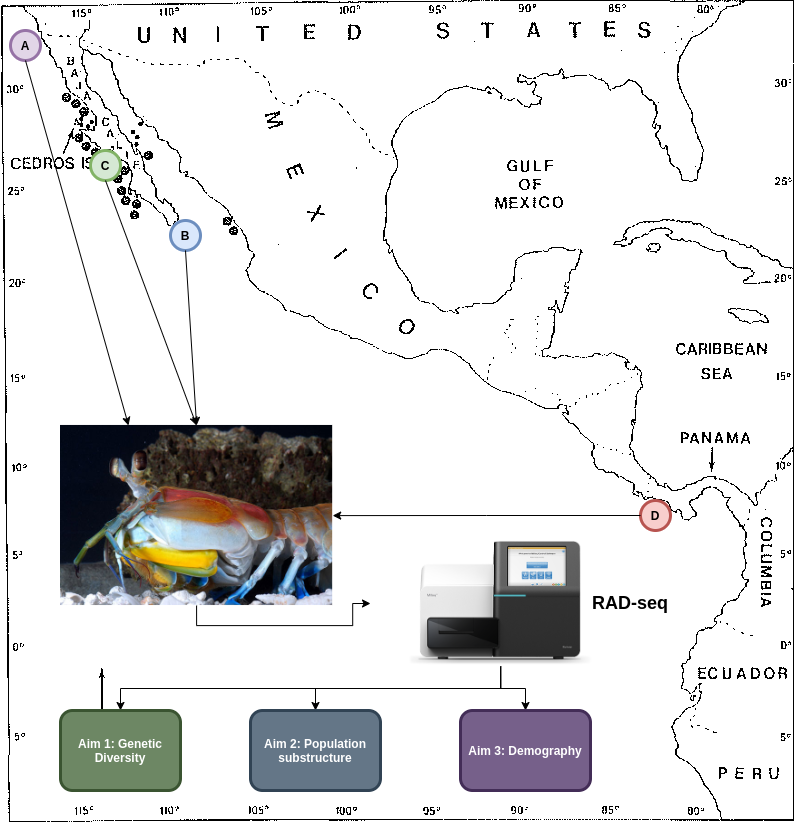
\includegraphics[width=0.30\textwidth]{images/sampling_locations.png}
	\end{center}
	\caption{Proposed \emph{Hemisquilla californiensis} collection locations shown as colored dots. Image adapted from \emph{Basch et al, 93}}
\end{wrapfigure}

Therefore, our main goal is to quantify genetic diversity of \emph{O. scyllarus} across their Atlantic range in order to access gene flow between populations and infer effects of recent antropogenic changes to the marine ecosystem by evaluating \emph{O. scyllarus} demographic and selective events. Towards this effort we will pursue three specific aims.

\section*{Aim 1: Characterize genetic variation.}

Genetic data will be gathered used restriction site associated DNA sequencing (RAD-seq) \cite{rad2011} which will allow the low-cost genotyping of a large number of individuals. RAD-seq libraries will then be used to calculate population level statistics useful towards accessing gene flow between populations namely pairwise inbreeding F-statistics. To quantify genetic differentiation   

This needs to be more about D and that kind of thing 

Genetic diversity lecture 13 notes is a good place for this.

\section*{Aim 2: Quantify \emph{O. scyllarus} population sub-structure.}
Hypothesis: \emph{Odontodactylus scyllarus} will show significant gene flow between sampling locations. Previous studies examining genetic variation of \emph{Oratosquilla oratoria}, a Mantis shrimp species closely related to the California Mantis shrimp, in the Yellow and East China seas found a surprising degree of gene flow between populations as determined by pairwise F\textsubscript{st} evaluations \cite{Yang2018}. However, it is currently unknown if Baja and Pacific \emph{O. scyllarus} exhibit similarly high levels of gene flow. To evaluate this question, we will collect \emph{O. scyllarus} individuals from four main locations; three along the the Western coast of Baja California, and one on the Western coast of Panama which is believed to be \emph{O. scyllarus} most Southern range. This will allow for comparisons to be drawn about the degree of gene flow between Northern and Southern populations. Using RAD-seq data collected in aim 1, we will calculate population level statistics useful towards accessing gene flow between populations namely inbreeding F-statistics. First we will determine reductions in heterozygosity due to genetic differentiation between the sampled populations by calculating the pairwise F\textsubscript{st} values. Ultimately F\textsubscript{st} is evaluated against the expected heterozygosity of the sub-populations if they were merged, had equal size and were randomly mating. Additionally, F\textsubscript{st} assumes Hardy-Weinberg equilibrium of the evaluated populations in order to access the heterozygosity from allele frequencies calculated from genotypic data. We will evaluate error in our estimations through permutation testing, which repeatedly randomly assigns individuals to a sub-population and evaluates  F\textsubscript{st} to ultimately create a probability distribution which can then be used to evaluate the significance of our actual results. 

We will further evaluate sub-population structure using a Bayesian approach to sub-population assignment. This method assigns individuals to a sub-population given their genotype and the allele frequencies of each sub-population under the assumption of a lack of linkage disequilibrium (all loci are treated as independent). Since the origin population of each individual is known, predictive capacity can be assessed to determine this kin

Last thing here could be admixture analysis which need to watch these videos about


MAybe change this to admixture analysis 

\section*{Aim 2: Evaluate sub-population structure within sampling locations}
Mantis shrimp species are known to be mostly solitary creatures, rarely spending significant amounts of time outside of their sea floor burrows \cite{Mead2010}. This small range is expected to give rise to significant population sub-structure within the four sampling locations. 


\begin{itemize}
	\item Fixation Index: reduction in genetic diversity of sub populations due to differentiation among sub populations.
	\begin{itemize}
		\item Access the reduction of differentiation to compare specific sub-populations using pairwise comparison. 
		\item How to define different sub populations? Blobs of areas / habitats
		\item High pairwise Fst to gauge the distinctness of populations. Do something where defining subpopulations 
		at greater and greater distances to determine how quickly Fst will drop off at different sampling sites. 
	\end{itemize}
	\item Another entry in the list
\end{itemize}



Expected heterozygotes Ht (total population was randomly mating)
Collect genotype data from a single locus A/T SNP and collect
adults 
Determine allele frequencies of locus interested in
This is where would look at mean Fst (fixation index which is mean reduction in Hs (expected heterozygotes due to genetic differentiation among sub-populations)).
Fis (inbreeding coefficient reduction in Hi due to non-random mating within a sub-populations )
Bayesian sub-population assignment 
possibly admixture analysis here as well

Change this whole thing to house cats vs feral cats and outgroups to see and selection subpopulations will make more sense since could look across different neighborhoods in chicago and see population
structure and more of a river type of thing so I am going to go with that.

\section*{Aim 3: Determine demographic history between Northern and Southern California Mantis shrimp populations.}

Hypothesis: \emph{O. scyllarus} will display a higher coalescent effective population size than instantaneous effective population size due to recent ocean acidification. 

Same magnitude of genetic drift as the actual population (Wright Fisher population)

Evaluate the effect of selection on the observed site frequency spectrum gleaned from RAD-seq data collected as a part of aim 1 by evluating the allele frequency selection of each suitable locus compared to the allele frequency spectrum of all other suitable loci across the genome. 

Would expect this to be demographic event though since fast maybe too extreme? This article suggests that 

For colensent need Pi and possibly mutation rate.

Instantous assumes constant size (wright fisher population) instanous effectice size is the same
as the coalsenset size (same amount of drift and genetic diversity Pi is colasent effective size) need a mutation rate as well to estimate this.

Expected Pi is average pairwise nucleotide differences this is also called theta for some reason
the larger a population is the larger we expect pi to be. Need to pick a specific locus and determine the number of nucleotide differences Pi is also tajima's theta which is an estimate of population size given a mutation rate. 

Ocean acidification would not effect mantis shrimp because did not really affect their weapons
https://www.nature.com/articles/srep38637

Evaulatue if selection acting differently on different populations 

\begin{itemize}
	\item How to tell demography vs selection?
	\begin{itemize}
		\item Wright-Fisher model predicts something. Neutral expectation. Constant size and no selection.
		\item Selection
		\begin{itemize}
			\item Selective sweep
			\item negative selection
			\item balancing selection 
			\item Any of these is occurring at specific loci that is under selection compared to a population (demographic level) change that should be observed genome wide because not specific to specific locus. 
		\end{itemize}
		\item Historical demography of a population
		\begin{itemize}
			\item Step 1 determine allele frequency spectrum of a population by sampling individuals and determine what that is 
			\item Neutral site freq spectrum has predictable decay but when looking at actual population and determine allele freq spectrum which might differ greatly from neutral expectation
			\item Step 2 is build some demographic model
			\begin{itemize}
				\item Pop size on y and time on x axis
				\item Shows how population size has changed over time
				\item s is the strength of the decline (or more generally the change in population size)
			\end{itemize}
			\item Step 3 Determine the parameters that we are going to vary
			\begin{itemize}
				\item Might want to determine the
					\item Strength of decline
					\item Timing of decline
					\item Rate of expansion
					\item Some combination
					\item These are the things that we are trying to determine. 
			\end{itemize}
			\item Step 4: Simulate data with different model parameter values.
			\begin{itemize}
				\item Get a simulated SFS sSFS
				\item DO many many simulations where you change the variables of interest and compare simulated SFS to observed SFS to try and find the parameter valeus that produce a simulated SFS to the population we are interested in.
				\item This is ABC approximate Bayesian computation
				\item Requires defining a prior distribution that will define the parameter space
				\item Simulate with the same amount of data that
				we collected and get gene copies sequences (simulated) which allows for calculating the
				simulated allele frequency spectrum 
				 
			\end{itemize}
		\end{itemize}
	\end{itemize}
\end{itemize}

5038141913


\pagebreak

\bibliography{refs}

\end{document}
